\begin{quoting}
\todo[inline]{Find a nice quote here}
\end{quoting}

Nowadays the vast market of mobile and embedded devices grows much faster than a traditional PC or server markets. With many more new use cases implemented and researched, one can speak about an explosion in a number of devices, their security requirements and security models. In order not to get lost in this constantly evolving variety, it is important to define a generic platform security model that can be used for classifying different types of platform security mechanisms and techniques, as well as compare platform security architectures between each other. 

Publication I of this thesis, as well as additional Publication VII (not included in this thesis) based on it, focus on creating this platform security model and comparing existing mobile platform architectures based on it. At the time of writing, mobile platforms were the most prominent direction for the OS platform security research and this explains the focus of the publications. The platform security model, defined in Publication VII is build on top of a set of common design patterns described in Publication I. These include hardware-assisted security mechanisms (secure boot, trusted execution environment, sealing and attestation, etc.) described in Section III, as well as software-only security mechanisms (protection of application integrity, run-time access control and permission assignment etc.), discussed in Section VI. The history of many of these design patterns go back some decades ago and they are constantly reused in newly coming platform security designs as "best known method" to fulfill a certain set of security requirements. For example, the "\textit{measure-before-execute}" design principle that is a foundation of the secure boot mechanism is a robust method to ensure that the software boot chain is free from offline (potentially malicious) modifications. Moreover, the first efforts to define and use hardware-assisted security mechanisms in platform security designs go back to late 1990s when the Trusted Computing Platform Alliance (TCPA)~\cite{pearson2002} defined first hardware-assisted elements for PCs.

There are four different mobile platforms that are discussed in Publication I: Symbian, Java ME, Android and MeeGo and this set is further extended to six in Publication VI by adding iOS and Windows Phone to the comparison. All of these platforms are compared in terms of security mechanisms they support, both hardware-assisted and software-only. However, as history has shown, only two of these mobile platforms have managed to reach significant device volumes in modern days, namely Android and iOS (73.5\% and 19.9\% of mobile market share respectively~\cite{osshare}). \todo[inline]{here tell about Android and iOS changes since} 

However, as we extend our focus to the world of embedded devices, the situation is different: there are no more software platforms or OSes that dominate this market. This is due to a very different nature of how embedded devices are designed and produced by OEMs, as well to a much wider set of use cases that such devices must support, such as automation, automotive, healthcare etc. A typical embedded device is usually a single purpose device, i.e. light sensor, garage door controller, factory supervision drone, but depending on the purpose has very different hardware and software stacks. For example, a device might need to interact with a user and therefore require a user interface or it might not need one at all. Similar with other technology support, as TCP/IP networking, Bluetooth, wireless, etc. 
Thus there is no a single ready-build OS that would serve as a good fit for all of these different purposes without causing an overhead of unnecessary components and instead in the embedded world it is more common to have "\textit{an OS-building set}", such as the ones provided by Open Embedded~\cite{OE2017} or Yocto projects~\cite{yocto2017}. Such sets are usually based on top of mainline Linux OS (both for the OS kernel and for userspace packages) in order to minimize the maintenance cost, because stable mainline Linux projects usually take a good care of keeping their components up-to-date and functioning with the rest of mainline Linux infrastructure, as well as doing various bug fixes and new feature requests. Using such an OS-building set allows even smaller OEMs to deliver their devices fast to the market, which is crucial for their business model. 

When it comes to security, the above trend means that the platform security architectures for embedded devices are mostly composed out of mainline Linux kernel security mechanisms that are used as building blocks to satisfy the set of security requirements for a concrete device. Some bigger OEMs might extend these mechanisms by adding their own private solutions, but it is not common due to high price of maintaining such solutions outside of the rapidly changing mainline Linux kernel source code tree. Following the model presented in Publication VI Figure~\ref{fig:platsec} shows the platform security architecture model that is applicable for any device that would only use the mainline Linux kernel components. Similar to the mobile platform security architectures, one can identify a set of well-known design patterns that these different mechanisms follow.


\begin{figure}[t]
	\centering
		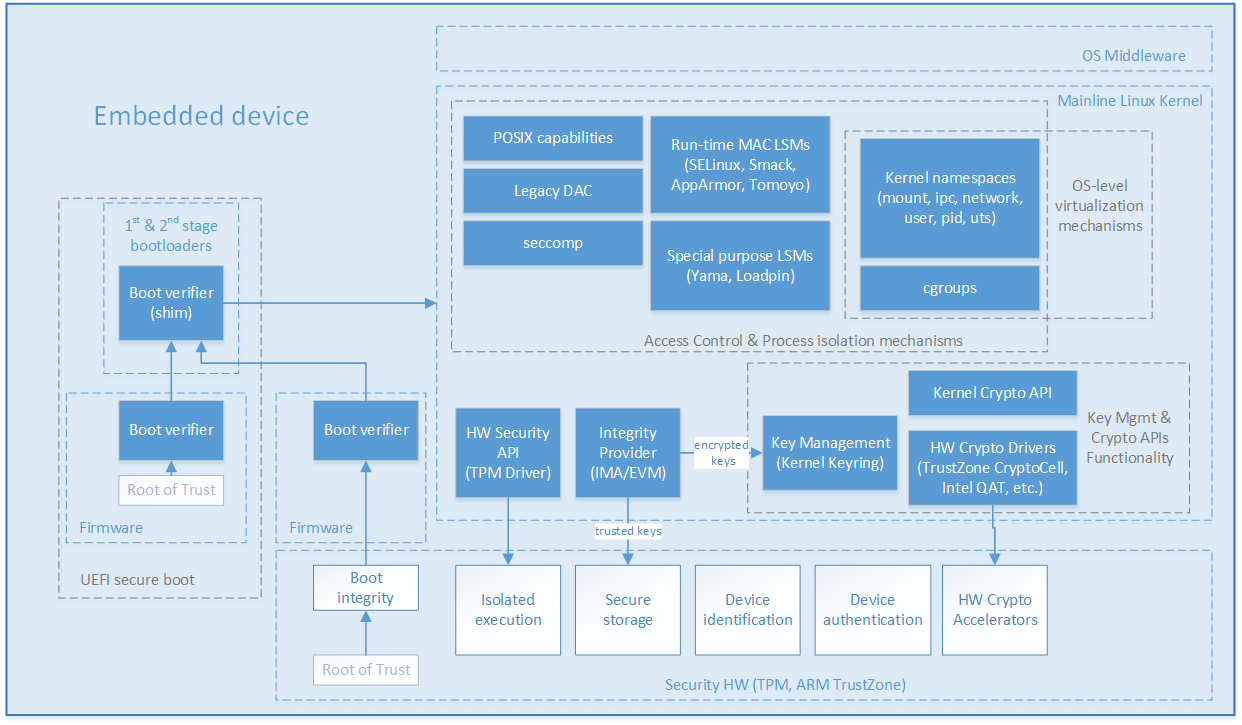
\includegraphics[width=1\textwidth]{figures/LinuxKernelPlatSecModel.png}
	\caption{Platform Security Model for an Embedded device based on mainline Linux}
	\label{fig:platsec}
\end{figure}


\todo[inline]{explain all the security components and their high level purpose}

Out of all design patterns described above, the run-time access control (required for process and application isolation) is the hardest one to configure and use correctly. Not only the mainline Linux kernel has multiple (and not excluding each other) options, such as traditional UNIX DAC, various MACs, kernel namespaces, POSIX capabilities, seccomp, but each of these options provides unlimited ways of how it can be configured. This is very challenging given that the end security of such mechanisms fully depends on its configuration or a policy, which might be at best provided for some of them only in a reference policy form and only for a certain use case. For example, there is a SELinux reference policy for Fedora desktop that only covers the packages included in the Fedora distribution, but as soon as new packages are added or substituted (common in the case of embedded devices), the policy needs adjustments and additions. Therefore the first main focus of this thesis, described in Chapter~\ref{sec:ac-policies}, is the methods for process isolation and access control, where we will take a look on the typical challenges of building secure MAC policies, as well as propose methods and tools that can help in this process. We will also focus on alternative methods for achieving process and application isolation using OS-level virtualization methods (kernel namespaces). 

In addition to the above described mechanisms, there is an area that recently gained a lot of focus in the mainline Linux security community, namely OS kernel protection against run-time exploits. The importance of this direction cannot be underestimated since a successful attack on the OS kernel itself renders all of its security mechanisms ineffective and useless. Therefore the second main focus of this thesis, described in Chapter~\ref{sec:kernel-hardening}, is OS Kernel Hardening, where we will discuss about overall ways to enhance the run-time exploit protection of the mainline Linux kernel, as well as presenting concrete mechanisms for achieving this goal. 
 